\vspace*{-5mm}
\mysection{Architectural Design}

\mysubsection{Overview}
In this chapter we will analyze the proposed architecture and components of the Travlendar+ system.\par
The proposed architecture is composed by three tiers :
\begin{itemize}
	\setlength{\leftskip}{0.5cm}
	\item \emph{Presentation Tier : }it's represented by Browser and Mobile App, the View part of our system.
	\item \emph{Web and Business Tier : }it's represented by Web Server, which responds to the user's HTTP requests, and Application Server, which contains all the Business Logic.
	\item \emph{Database Tier : }it's represented by DB Server, that contains and manages persistent data in an efficient way.
\end{itemize}
\begin{figure}[H]
	\centering
	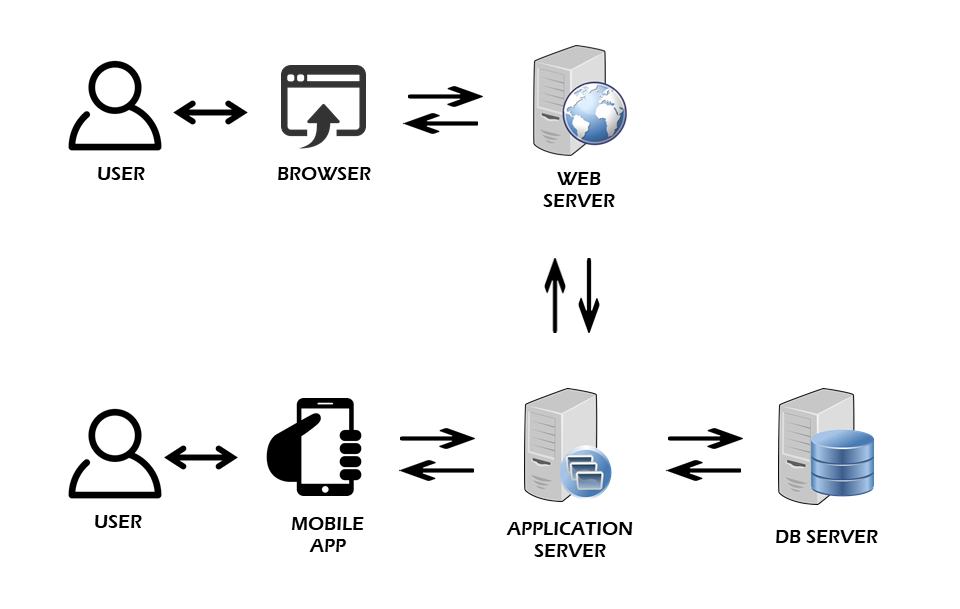
\includegraphics[scale=0.4]{Images/Architecture/Proposed_Architecture}
	\caption{Proposed Architecture}
\end{figure}

\mysubsection{High Level Components and Their Interactions}
\begin{figure}[H]
	\centering
	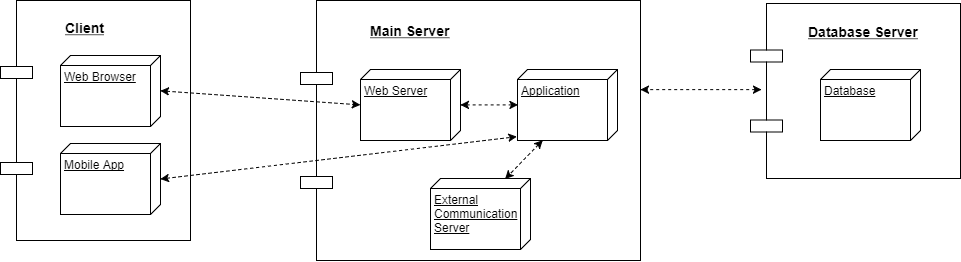
\includegraphics[scale=0.4]{Images/Architecture/Components_High_Level}
	\caption{Components High Level}
\end{figure}

\textcolor{red}{The system is divided in three main layers: Presentation Layer, Business Layer and Data Layer.
The presentation layer is both a web-based application and a mobile application. For the web application we will have a very thin client with the only aim of performing requests, through a web server, to the Business layer and receiving the HTML pages with the demanded information.
On the other hand, the mobile application will not require an interface with the web server because it will communicate directly with the server.
The main server is composed by three parts : the Web Server, 
Our system, being a calendar based application, will have the main issue of managing a richly structured body of information. In our case these information will be persistently stored in multiple Data Bases, each one containing a precise schema with a precise kind of data, and they always have to reflect the true state of affairs. For this reason every client's requests that will implicate a changing data operation is preceded by a set of controls performed by defined control components designated to the database’s consistency maintenance.}

\mysubsection{Component View}
\begin{figure}[H]
	\centering
	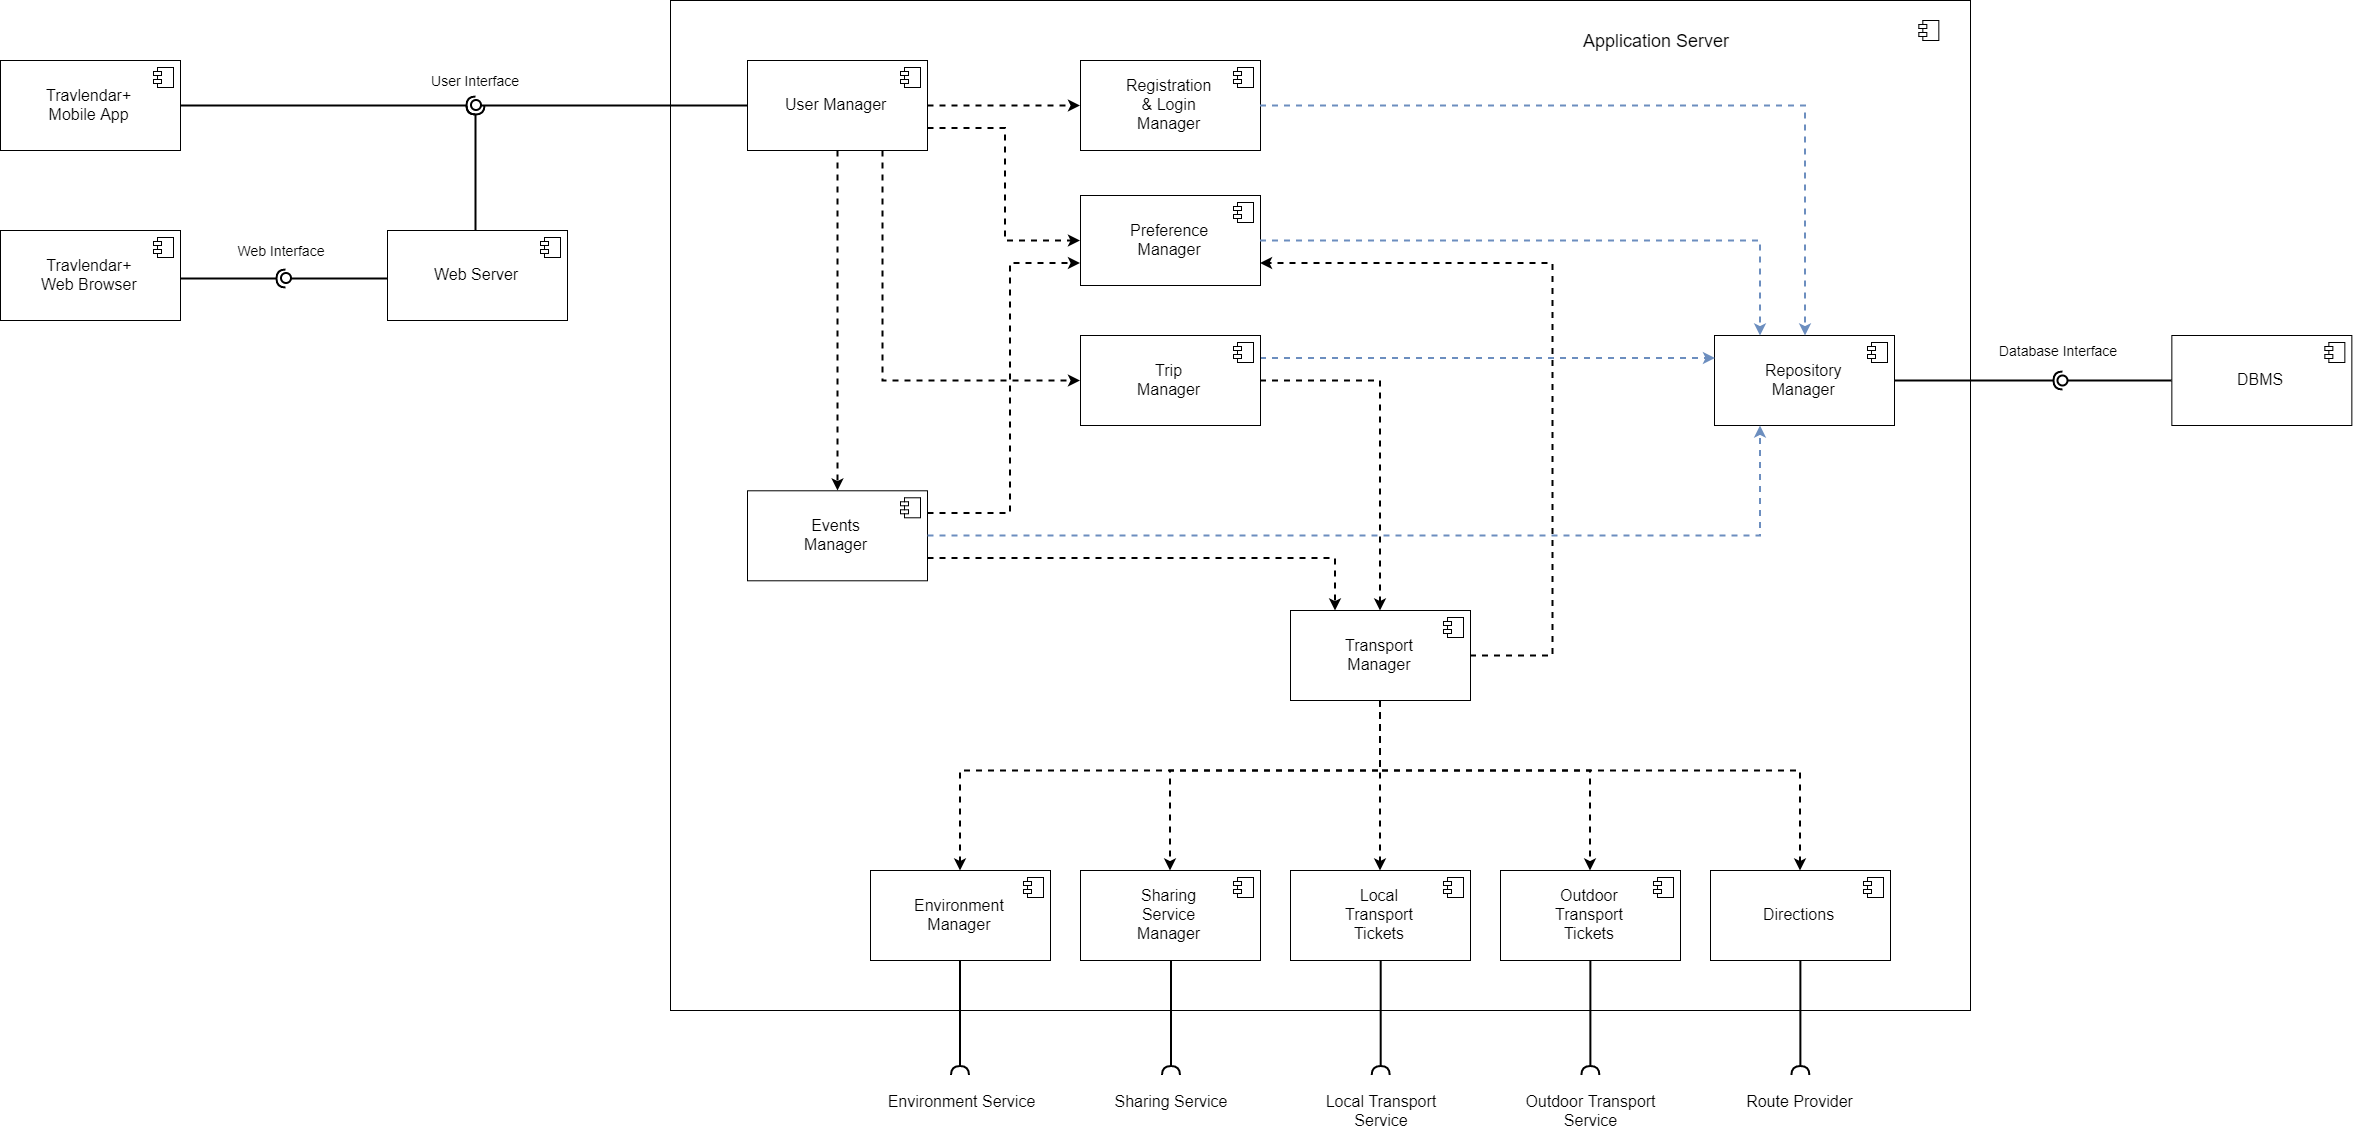
\includegraphics[scale=0.17]{Images/Architecture/Components_View}
	\caption{Component View}
\end{figure}
\mysubsubsection{Travlendar+ Mobile App}
This is the component responsible for the communication between user’s devices, like user’s smartphone, and the rest of the system. It will exchange REST messages with the \emph{userInterface} and will render the  based on the server’s replies.\par
In order to communicate with the server the component will use specific frameworks and libraries depending on the specific device used by the user (ex. Android SDK Platform for Android smartphones).\par
This component represent the View part of our MVC pattern.

\mysubsubsection{Travlendar+ Web Browser}
This is the component responsible for the communication between user's browser and the rest of the system.\par
It sends HTTP requests to the \emph{webInterface} in order to get back from the server HTML pages and static resources like CSS and JavaScript files.

\mysubsubsection{Web Server}
This component is responsible for the HTTP responses of the \emph{webInterface}. Its main function it’s to elaborate pages, generate contents in a very dynamic way and send them to the browser. These processes are performed by the Web Server instead of the user's Browser for managing in the most efficient way the user CPU's load.\par
An example could be the Apache HTTP Server. It’s cross-platform, highly scalable and use a \emph{gzip} module to reduce web pages size (weight).

\mysubsubsection{User Manager}
This is one of the most important component of the server because it handles the communication with the user, so it takes care of all possible breakouts or errors that may occur runtime. It also manages all user’s request redirecting them to other server’s specific components.

\mysubsubsection{Registration \& Login}
It allows user to register and login to the system memorizing and verifying user’s credentials.

\mysubsubsection{Preference Manager}
It allows user to set all his preferences such as carbon footprint, TAGs, residence location, etc… So its aim is to memorize these preferences’ data in the DB through the Repository Manager and get them every time is needed.

\mysubsubsection{Trip Manager}
This component handles all user’s trips, allowing him to add, delete or edit trips. It allows also the user to buy tickets to reach the trip’s location (through the Outdoor Transport Tickets component) and tickets to use the local transport service in the destination city (through the Local Transport Tickets).

\mysubsubsection{Events Manager}
This component takes care of user’s calendar managing the events that the user wants to add, delete, edit or visualize.\par
So every time he wants to :
\begin{itemize}
	\setlength{\leftskip}{1cm}
	\item \emph{insert or edit an event}, this component will check through the Repository Manager if in the DB there is an overlap and if the event is reachable from the previous one (using also Transport Manager to verify route’s time).
	\item \emph{delete an event}, this component will simply delete it in the DB.
	\item \emph{visualize an event}, this component will check through the Transport Manager the available means of transport, the time needed and the route to reach the event.
\end{itemize}

\mysubsubsection{Transport Manager}
This component handles all event’s means of transport and tickets. About transport, it filters the means according to :
\begin{itemize}
	\setlength{\leftskip}{1cm}
	\item the means selected in the event’s TAG;
	\item the $CO_2$ preference;
	\item the means selected in the “Available Means” in Preferences;
	\item the means available to reach the event (received by the route provider);
	\item the weather conditions;
	\item the strikes.
\end{itemize}
It allows also to buy local transport tickets if the user needs to. 

\mysubsubsection{Directions}
This component handles the communication with the route provider in order to get maps, means and routes to reach a specific destination. To get these information it uses API requests (an example are Google APIs).
It also parses and elaborates the API responses in specific structures in order to allow the other server’s components to use them in the best way.

\mysubsubsection{Environment Manager}
This component is used by our system to check and warn the user about the weather's conditions and the transport strikes.
It uses API requests in oreder to communicate with the external services.

\mysubsubsection{Sharing Service Manager}
This component allows our server to communicate with external sharing services in order to get the nearest sharing mean of transport's location.

\mysubsubsection{Local Transport Tickets}
It takes care of the communication with the local transport services for getting information about the available tickets, suggesting to the user the best one to buy based on his travel's needs.

\mysubsubsection{Outdoor Transport Tickets}
It takes care of the communication with the outdoor transport services in order get information about the available tickets and means of transport.

\mysubsection{Deployment View}

TEXT HERE

\mysubsection{DB Structure}

INSERT DBMS DIAGRAM

\mysubsection{Runtime View}

TEXT HERE

\mysubsection{Selected Architectural Styles and Patterns}

\textcolor{red}{\huge mettere spazio fra i paragrfi}\\
Our system architecture proves to be a mix between three well known architectural styles, in particular : 

\begin{itemize}
\setlength{\leftskip}{0.5cm}
\item \emph{Client/Server Architectural style}
\item \emph{Main program with subroutines architectural style}
\item \emph{Service oriented Architectural style}
\item \emph{Event Based Architectural style}
\end{itemize}

The system is divided in three main layers: Presentation Layer, Business Layer and Data Layer.
The presentation layer is both a web-based application and a mobile application. For the web application we will have a very thin client with the only aim of performing requests, through a web server, to the Business layer and receiving the HTML pages with the demanded information.
On the other hand, the mobile application will not require an interface with the web server because it will communicate directly with the server.

The main server will contain all the logic of the system. The main component of the logic will be the User manager. This component will perform as the Main program in the Main program with subroutines style: it will receive the requests from the clients and call the right sub-component for accomplishing the goal related to the request.

Our system, being a calendar based application, will have the main issue of managing a richly structured body of information. In our case these information will be persistently stored in multiple Data Bases, each one containing a precise schema with a precise kind of data, and they always have to reflect the true state of affairs. For this reason every client's requests that will implicate a changing data operation is preceded by a set of controls performed by defined control components designated to the database’s consistency maintenance.

if the requests will pass the check steps a special component called Repository Manager is activated. This component will offer function that performs all the operation that change the DBs’ state with an high level of abstraction. In fact these methods will be constituted by a composition of DBMS operation that accomplish the aim of the requests: in this way the complexity of articulated DB operation is hidden to the caller and is very simple to add new methods making this interaction highly scalable.

An essential our system business, as said in the RASD, will be to provide directions related to the precise travel means, sharing means’ position and give tickets information about local and outdoor public transport. All these information will not be stored in our DBs, but they will be retrieved with API REST requests to fitting external services. For this goal we will use a SOA style. 
In our system we will have a component called Transport manager that will be able to distinguish the kind of the request and demand the aim of submitting it to the right external service to another precise component devoted to a certain type of external services connections. Once received the information, their manipulation will be performed internally to the business logic of the system. In these way we will have the possibility of adding new components for incoming kind of transportation, also personalized, in a very simple and scalable way.

The last style exploited is the Event based Architectural style, and it is used for the notification system always attending particular events that, if happens, triggers the component that produce a notification that is immediately sent to the right client. 

\mysubsection{Design patterns}

\begin{itemize}
	\item 
\emph{MVC}: The Database server contains all the software’s data and constitutes the model part. The presentation layer with the web-based application and the mobile application is the view that is released to the user. Finally the main server,  that is the business logic layer, it’s the control part.

\item \emph{OBSERVER:} Our software has to be able to, for instance, advising the user that he has to take a certain mean in a specific time for arriving on time, or that the registered season ticket is expiring or also the possibility of a strike or a bad meteorological condition. All these events have to be supported by a notification system.This needs will be implemented with this pattern.  There will be a specific group of event listener, namely objects that extend a common abstract class. When a process that could generate a notification starts, one or more concrete references of event listeners are got by the objects involved into the process devoted to perform operations and eventually change the variables, or a set of variables of interest. The system will have as much kind of event listener as is necessary and they could be added freely for future expansion. When during such a process a variable of interest for a listener is changed some checks are performed and, under some particular conditions, a notification is created and sent to the user. 

\item \emph{STRATEGY:} The filters applied on the data for showing particular results based on the user’s choices, for example for advising the best means of transport for a destination, will be implemented with a strategy pattern. The class the will put in order the results will have an instance of an abstract class that will be implemented by some concrete class representing different ordering strategy. In this way the system will be able to adapt his strategy runtime and it will be very simple to add new strategy creating new classes that will implement the abstract strategy class previous mentioned.

\item \emph{COMPOSITE:} We will use this pattern in our system for performing in a cleaned and elegant way the various check that will have to be apply on the user input. There will be a abstract class Checker that will be extended by Composite checkers and Checkers. Each composite checker contains one or more checkers and both implements the method check. The class that will have to manage a specific user input will have one or more composite checkers.
When a method that have to process the user input data for passing them to an external service or to another component that will insert such a data in a DB, the check method of all the compiste checker in such a class will be called and each composite checkers will recursively call his checker’s check method. In this way all the check will be applied and if something is wrong, the subsequent operation will not be executed and all the possible problems linked with that will be avoided. 
Thanks to this pattern is possible to create new checkers/composite checkers very easily and deal with complex and composite check that will be needed in future software expansions.

\item \emph{FAÇADE:} As guideline of our implementation, for all the complex operations that will require multiple method’s calls from different classes we will use a façade pattern. In this way we will able to hide a complex logic operation within a single method’s call. In this way we will simplify the software maintenance for future changing needs.
\end{itemize}

\mysection{Algorithm Design}
A very delicate phase of our system is that one in which the user input is checked. This is so important because the most user’s operations in Travlendar+ terminates writing data on the Data Bases and if the system letted wrong input to be written in the persistent memory, will rise big problems of inconsistency.

The operations that the user is allowed to do, work all with similar data but the checks that have to be performed are different, sometimes very complex and also some of them need a check’s combination concerning single operations.

Moreover, giving a quick look on the rapid world’s evolution, it sounds quite possible that new kinds of event and operations could be implemented in the system and so we needs that create a modular and scalable way of facing this problem is a issue of primary importance.

We will take on this problem using the composite pattern, that has been described item by item in the design pattern paragraph. We give downward an example of how will be implemented a checking process from the received request to the writing of the data into the DB.

\emph{ \huge CONTINUARE CON SCREEN DELL'ALGORITMO SPIEGATO}

\mysection{Implementation, integration and test plan}
In this section we will give a plan that we have projected for implementing Travlendar+. 
Firstly we will give the strategy for the processes chosen for taking on the our project and the structure of our team, how it is divided and the tasks that each part has to accomplish.
After we will state how each team’s part has to interact with the others and the span of time of these interactions. 
Finally we will give a list of possible risks, the probability that they happen, their impact and a possible strategy to deal with them.

\mysubsection{Strategy adopted}
For giving a quality assurance of the project and be sure that the product will be as our stakeholders expect, we will an Agile planning process. It consists in a first initiating part in which it’s given an overall plan of the system process. 
We have started with the information given in the RASD and we will terminate it in this document: in fact we have already stated the software’s architecture and the design pattern that will be used and in this section we will give a schedule for all the various' team tasks.

After this part, there is a cycle of phases called respectively: Executing, monitoringANDControlling, Closing, Planning. 
Every cycle round has as input a specific process to accomplish, divided between the various team’s parts. After executing all the task in a precise given timeframe, the works is checked and after the parts agreement, that is reached after that the customers have analyzed the results, it will follow another planning phase that will contain also the corrections that will result after the agreement.
This cycle is repeated until the end of the project, when all the functionalities stated in the RASD will be covered.

\mysubsection{Team structure}
Our team will be composed by two main parts:

\begin{itemize}
	\item \emph{Developers :} people devoted to implement the software
	
	\item \emph{Testers: }people devoted to test the software functionalities
	
	\item \emph{Front-End Team :}developers appointed to implement the system’s front end.
	
	
	\item \emph{Back-End Team :}developers appointed to implement the application logic of the system
	
	\item \emph{Supervisors: }developers that belongs to the Back-End Team or to the Front-End Team and that have the main task of having any time the picture of all the their team work.

\end{itemize}

\mysubsection{Implementation and testing plan}

The work will be divided in sub-milestone from a minimum of one to a maximum of two weeks, and main-milestone every three or maximum four weeks. In these span of time all the teams have to complete the tasks that have been established in the previous planning phase. Every two days the different team's supervisors and a Tester’s team delegate will manage a meeting for speaking about their teams progress and will give directive for proceeding basically at the same speed. 
in the while, the Tester team will work on white-box test for the functionalities that the developer’s teams are implementing.
When the milestone’s day come, the Tester team will have from a minimum of a day to a maximum of one they for testing the functionalities and give the results to the development team that will have to fix the eventual bugs.

During the week before the the milestone’s day, the Tester team has to perform an integration test of the components and give the result to the development teams that has to release a beta version to restrict and selected group of people for the milestone day. In this way, will be performed also an incremental User acceptance test on the work that has been done. 

\mysubsection{Possible risks}
\emph{ \huge NON LO SO METTERE BENE}
		Probability		Effects
		Budget problems		L			Catastrophic
		
		Time                                    M                            Serious
		for implementing 
		a function exceed
		from the calculated one
		
		Team’ members                  M                            Catastrophic
		not available in critic
		moments
		
		Impossibility to recruit          M                           Serious
		staff with required skills  

\mysubsection{Possible solutions}
\begin{itemize}
	\item \emph{Budget problems :}specify before starting stating all the functionalities a realize prevision of the costs predicted and agree with the stakeholder a margin of budget that could increase for unpredicted situation during the development.
	
	\item \emph{Time for implementing a function exceed :}agree with the stakeholder a span of time of delay that they can accept for unpredicted problems.
	
	\item \emph{Team’s member not available in critic moment :} being sure that at least one of the supervisors could substitute a team member in case of necessity
	
	\item \emph{Impossibility to recruit staff with required skills :} advices the customers about possible delete and be ready with a list of COTS to buy in case of needs with the correspondent costs.
	
\end{itemize}
